Hallar el área de la región acotada por $y=5-|x|$, el eje $x$ y las rectas $x=-5$ y $x=5$.

\nopagebreak
\begin{align*}
\text{La función es par y simétrica respecto al eje } y. \\
\text{Intervalo: } [-5,5]. \text{ Podemos calcular } 2 \int_{0}^{5} (5-x) \, dx. \\
\text{Suma de Riemann (para } [0,5]\text{): } \Delta x = \frac{5}{n}, x_i = \frac{5i}{n}. \\
A = 2 \lim_{n \to \infty} \sum_{i=1}^{n} \left(5 - \frac{5i}{n}\right) \frac{5}{n} \\
\text{Evaluando geométricamente (triángulo base 10, altura 5):} \\
A = \frac{1}{2} \cdot 10 \cdot 5 = 25 \\
\text{O por integral: } \int_{-5}^{5} (5-|x|) \, dx = 2 \left[ 5x - \frac{x^2}{2} \right]_{0}^{5} \\
= 2 \left( 25 - \frac{25}{2} \right) = 2 \left( \frac{25}{2} \right) = 25
\end{align*}

\[
\boxed{\displaystyle 25}
\]

\begin{center}
    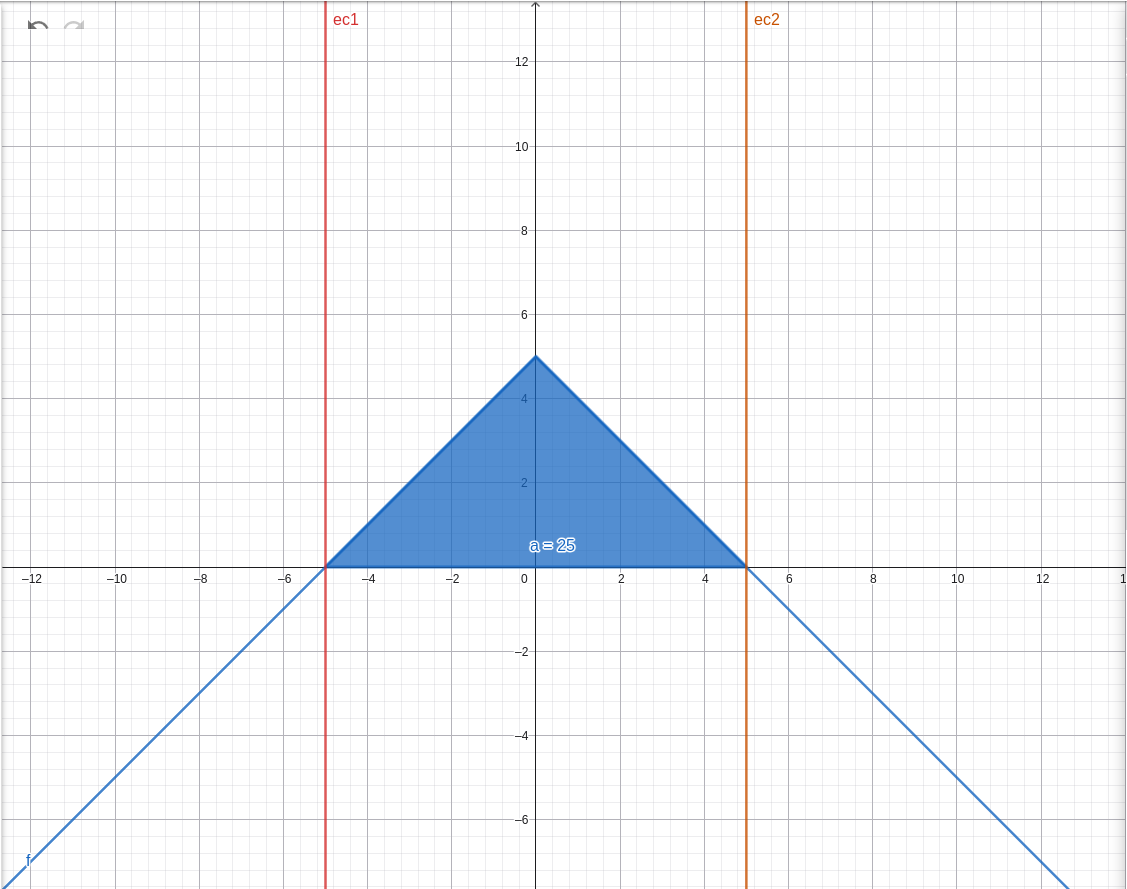
\includegraphics[width=0.5\textwidth]{Graficas/ejer10.png}
\end{center}
